\chapter{Literature Review}

This chapter will provide a review of the existing literature, which will be used guide the student in their planning and development efforts of the project.

\noindent As such, it will be covering the following areas:
\begin{itemize}
    \item Healthcare-specific research
    \item Software development methodologies
    \item Requirement gathering
    \item Tech stack
    \item Large Language Models (LLMs)
    \item PHR Systems
\end{itemize}

\section{Software development methodologies}

\subsection{Software Development Life Cycle}

The Software Development Life Cycle (SDLC) is a process used to guide the development of software applications or systems \parencite{sdlc1}. The SDLC consists of multiple phases, each with its own set of activities and deliverables. \textcite{sdlc2} outline the phases of the SDLC as following:
\begin{enumerate}
    \item Requirement gathering and analysis phase - the requirements are gathered from the project stakeholders and saved in a specific document. Based on the requirements gathered, a development plan is created and a feasibility study is conducted.
    \item Design phase - the previously gathered requirements are written in a more technical manner and system deisngs are created that will later guide the developers to develop the software. 
    \item Implementation phase - Actual development of the software occurs in this phase. Additionally, some smaller unit tests may be done during this phase as parts of the software are developed.
    \item Testing phase - may involve multiple types of testing, such as unit testing, integration testing, and system testing. \textcite{testing} describes the different types of tests as following:
    \begin{itemize}
    \item Unit testing - done on the lowest level of the software, testing individual units or components of the software.
    \item Integration testing - performed on two or more units combined together, usually focusing on the interfaces between these components.
    \item System testing - focuses on the `end-to-end quality of the entire system', testing it as a whole based on the system requirement specification.
    \end{itemize}
    \item Maintenance phase - involves the deployment and maintenance of the software. Additionally, this phase may include user acceptance testing, where the software is handed over to the end-users to ensure that it meets their needs \parencite{testing}. 
\end{enumerate}

\begin{figure}[ht]
    \centering
    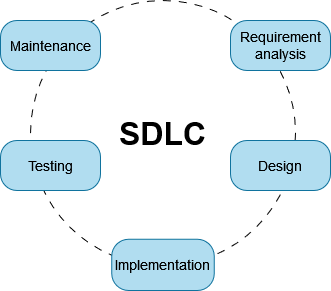
\includegraphics[scale=0.6]{SDLC.png}
    \caption{Software Development Life Cycle}
    \label{fig:sdlc}
\end{figure}

\newpage

\subsection{SDLC Models}

The literature describes several SDLC models that have been used in the development of software applications. \textcite{sdlc1, sdlc2} outline the most common SDLC models: Waterfall model, V model, Spiral model, Interative model, and Agile model.

\subsubsection{Waterfall Model}

The Waterfall Model is the most well-known SDLC model. It is a linear model, where the development process is divided into distinct, sequential phases.

The Waterfall Model's strengths lie in its simplicty of use, ease of understanding and a structured approach \parencite{waterfall}. An additional stregth of the Waterfall model that the authors note is its extensive documentation and planning, which is done in the early stages of a project, that is also maintened throughout the project. These two factors also help minimize the overhead that comes with planning and management of a project.

One of its main weaknesses, mentioned by \textcite{waterfall}, is its lack of flexibility in regards to change of requirements. Once the project leaves the requirements analysis or design phase, it may be difficult to make any changes to the project deliverable. Thus, this model is not suitable for projects where the requirements are not well understood or are likely to change. Finally, the deliverable is only available at the end of the project, so the end-users can provide any feedback during its development \parencite{waterfall}.

\begin{figure}[ht]
    \centering
    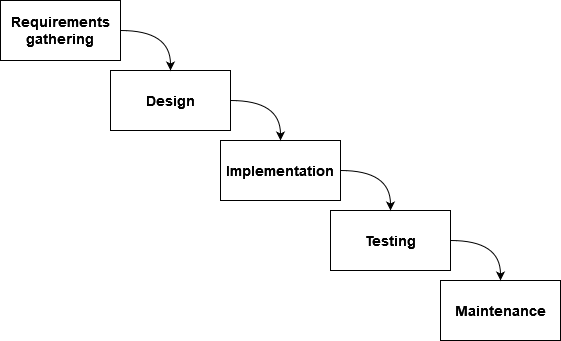
\includegraphics[scale=0.45]{Waterfall.png}
    \caption{Waterfall model}
    \label{fig:waterfall}
\end{figure}

\subsubsection{Agile Model}

Another well-known model is Agile. It focuses on the idea that requirements are not always well-known and accepting that change is inevitable \parencite{agile}. Similarly, as the author mentions, the focus of this methodology is on continuous delivery of software and interaction with the customer to get feedback. The author mentions that Agile is well known for its flexibility and adaptability to change, its ability to deliver working software in short iterations and its focus on customer satisfaction.

Agile has multiple frameworks that can be used to guide the development process, such as Scrum or Kanban. Scrum is an Agile framework, where the project is divided into sprints, each lasting between 2-4 weeks and focusing on delivering value to the customer through incremental software features \parencite{scrumban, agile}. On the other hand, Kanban focuses on visualizing the project workflow through a visual board by using columns, cards and swimlanes. Kanban's main goal is to limit the work in progress through column limits and a pull system to maximize the flow of work through the system \parencite{agile}.

Agile does have some drawbacks - its lack of documentation and formal planning, especially in the early stages of the project, may not be suitable for large scale projects, where extensive documentation and planning are required \parencite{sdlc1, agile, sdlc2}. Similarly, the Agile model may not be suitable for projects where the requirements are well understood or where there may be strict regulations that guide how the project should be developed.

Nowadays, the use of Scrum and Kanban together is becoming quite popular, with many teams employing both frameworks in their projects. As \textcite{scrumban} mention, this can be quite beneficial as it allows teams to adopt the appropriate practices of both methods and adapt them accordingly based on their needs.

\begin{figure}[ht]
    \centering
    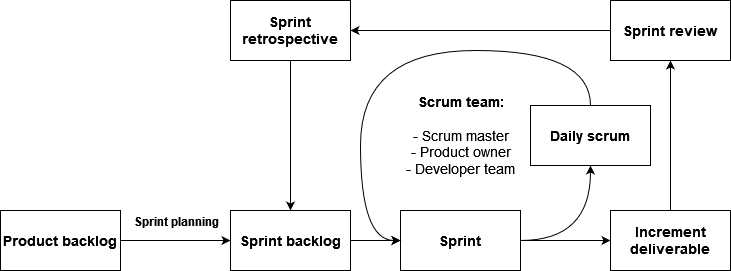
\includegraphics[scale=0.45]{Scrum.png}
    \caption{Scrum framework}
    \label{fig:scrum}
\end{figure}

\subsection{A hybrid approach}

For many years, Waterfall has been the most widely used model in software development projects, with Agile approaches gaining popularity in the recent years \parencite{hybrid1}. However, a hybrid approach has also been emerging, with various surveys reporting a combined approach being used in project work \parencite{hybrid1,hybrid2}. The most common combinations that form this hybrid approach are Scrum, Iterative Development, Kanban, Waterfall and DevOps, with the approach that combines Waterfall and Scrum being the most popular \parencite{hybrid2}. In that case, only the development part is usually done in an Agile way - with the rest of the project using the traditional approach as a backbone \parencite{hybrid2}.

\textcite{hybrid1} note that projects using either Agile, traditional or hybrid approach show similar levels of success in terms of budget, time and quality. However, the authors have found that agile and hybrid approaches perform much better on the customer satisfaction metric than the traditional counterpart.

\section{Requirements gathering}

Regardless of the approaach used, the requirements gathering phase is the first step in any software development process. As described by \textcite{reqanalysis2}, a requirement is a `necessary attribute in a system\ldots that identifies a capability, characteristic, or quality factor of a system in order for it to have value and utility to a user'. Multiple studies mention how proper requirement gathering plays a pivotal role in the project quality and success, with a majority of project failures being attributed to poor requirements gathering \parencite{reqanalysis1, reqanalysis3, reqanalysis5}.

\subsection{Requirement types}

Requirements can be classified into 2 categories: functional and non-functional requirements. Functional requirements describe the system's behavior, such as what the system should do and how it will react to different inputs, while non-functional requirements describe the system's quality attributes, such as performance, security, reliability, etc. \parencite[6]{requirements}.

When writing the requirements in a document, it is important to ensure that everything is written in a clear and concise manner to avoid any ambiguity. As such, \textcite[112]{requirements} recommends using a standard format for writing all requirements: using simple language in a consistent manner, avoiding the use of technical jargon, vague terms and not creating multiple requirements in a single statement.

Similar principles of writing requirements can be found in \textcite{requirements2} which also provides a list of requirement characteristics: necessary, appropriate, unambiguous, complete, singular, feasible and verifiable. The same standard recommends using attributes to describe each requirement, such as an identification, owner, priority, risk, rationale, difficulty, and type (functional/non-functional).

Prioritizing requirements is another crucial task, especially in projects with numerous requirements. Some methods include using a low to high priority, assigning a numerical value within a specific range or MoSCoW, which classifies requirements into four categories: 
\begin{itemize}
    \item Must have - must be implemented in the software before being released
    \item Should have - important but not necessary for the software to be released
    \item Could have - desirable but not necessary for the software to be released
    \item Won't have - requirements that are not included in the current release
\end{itemize}

\subsubsection{Requirements in Agile}

In Agile projects, the most basic unit of requirements are usually written in the form of User Stories, which are simple descriptions of a feature desired by the customer \parencite[191]{requirements}. User Stories are written in a specific format, such as `As a [user], I want to [action] so that [benefit]'. Other components of a User Story include a title, acceptance criteria (conditions that must be met for the story to be complete), priority, story points (estimated time to implement), and description. Epics are larger user stories that cannot be completed in a single sprint. Epics can be broken down into smaller user stories, which are then added to the Product or Sprint Backlog.

Both Epics and User Stories are part of the Product and Sprint backlog - the former one containing the list of requirements for the whole project and the latter containing the list of requirements for the current sprint/iteration.

\subsection{Stakeholders}

Stakeholders represent the `set of individuals who have some interest (a stake) in the success (or failure) of the system in question' \parencite[34]{requirements}. The author stresses the importance of accurately identifying all possible stakeholders in the early stages of the project, as leaving out key stakeholder could lead to missing out on important requirements or constraints later on the project. 

After identifying the stakeholders, it is important to do a stakeholder analysis by understanding the stakeholders' needs, expectations, and influence on the project. One way of doing it is by using a stakeholder matrix, such as the Influence/Interest grid (see figure X), which classifies stakeholders based on their power and interest in the project \parencite{stakeholders}.

\begin{figure}[ht]
    \centering
    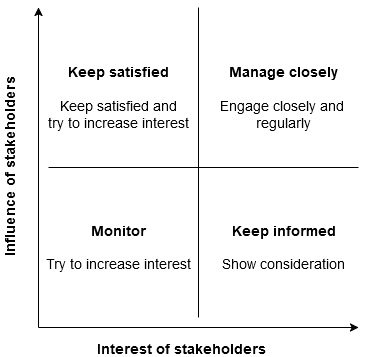
\includegraphics[scale=0.6]{Stakeholder.png}
    \caption{Stakeholder Influence/Interest matrix}
    \label{fig:stakeholder_matrix}
\end{figure}


\subsection{Requirement gathering techniques}

There are multiple requirement gathering techniques, the most popular ones being interviews, workshops, prototyping, modelling, brainstorming, storyboards and observing users \parencite{reqanalysis1,reqanalysis2, reqanalysis3, reqanalysis4}. One of the studies interviewed several individuals with multiple years of experience in the field of requirement gathering and analysis. As a result, the authors found that the most used requirement gathering techniques were collaborative meetings, interviews, ethnography and modeling \parencite{reqanalysis1}.

\subsection{Interview technique considerations}

Multiple research papers point to interviews being recognised as the most commonly used technique for requirement gathering \parencite{interviews5,interviews1,interviews2}. Additionally, some studies have looked at best practices and common mistakes when conducting interviews for requirement gathering - the results of which are summarized in the tables below.

\begin{table}[h!]
    \centering
    \small
    \begin{tabular}{|p{0.2\textwidth}|p{0.75\textwidth}|}
    \hline
    \textbf{Study} & \textbf{Recommended Practices} \\ \hline
    
    \textcite{interviews4, interviews3} & 
    \begin{itemize}
        \item Encourage deep thinking through situational thinking or rationales.
        \item Avoid ambiguity by asking clarifying questions.
        \item Be flexible by probing into relevant topics.
        \item Verify alignment with the customer's vision.
        \item Use projective techniques like scenarios or role-playing.
        \item Allow stakeholders to teach analysts complex topics.
        \item State goals at the beginning and allow customer input at the end.
    \end{itemize} \\ \hline
    
    \end{tabular}
    \label{tab:recommended_practices}
    \caption{Recommended Practices for Requirements Gathering Interviews}
\end{table}
    
    
\begin{table}[h!]
    \centering
    \small
    \begin{tabular}{|p{0.2\textwidth}|p{0.75\textwidth}|}
    \hline
    \textbf{Study} & \textbf{Common Mistakes} \\ \hline
    
    \textcite{interviews1} & 
    \begin{enumerate}
        \item Wrong opening: failing to understand the context before discussing the problem.
        \item Not leveraging ambiguity to reveal knowledge gaps.
        \item Implicit goals: failing to ask or clarify stakeholder goals.
        \item Implicit stakeholders: overlooking third-party stakeholders.
        \item Ignoring non-functional requirements.
        \item Wrong closing: skipping interview summaries or feedback.
    \end{enumerate} \\ \hline
    
    \textcite{interviews2} & 
    \begin{enumerate}
        \item Poor question formulation: vague, technical, irrelevant, or too long.
        \item Question omission: not asking about business processes or doing follow-up questions.
        \item Incorrect order:  incorrect opening (no introductions, no description of the current situation) or ending (no summary).
        \item Weak communication: too much technical jargon usage or not listening to the customer.
        \item Poor customer interaction: failing to build rapport.
        \item Lack of planning: unstructured sequence of questions.
    \end{enumerate} \\ \hline
    
    \end{tabular}
    \caption{Common Mistakes in Requirements Gathering Interviews}
    \label{tab:common_mistakes}
\end{table}    

\section{Tech stack}

\subsection{Database}

There are several types of databases, such as: relational (SQL), NoSQL databases, graph databases or object-oriented databases \parencite{databases2}. The choice of database depends on the project or organisation requirements, such as the amount of data, the complexity of the data, the need for scalability, etc. 

\subsubsection{Relational databases}

Relational databases store structured data in tables, linked through keys to create relationships between entries \parencite{databases}. They use SQL (Structured Query Language) to create queries and schemas to help organise and manage data efficiently. \textcite{databases} highlight that relational databases are used, thanks to their high data integrity, for industries like finance and healthcare. Relational databases are widely used and have a large community, making it easier to find support and resources. However, the rigid schema limits adaptability to rapid data changes, and scaling horizontally in distributed systems can be challenging. Examples include MySQL, PostgreSQL, Oracle, and Microsoft SQL Server.

\subsubsection{NoSQL databases}

NoSQL databases manage unstructured or semi-structured data without rigid schemas or relationships \parencite{databases}. As the authors describe, NoSQL databases, such as key-value, document, column-family, and graph databases, excel in flexibility and scalability. NoSQL databases often prioritize performance over strict consistency, making them suitable for large, varied datasets of unstructured data but less ideal for complex transactions. Although growing in popularity, NoSQL systems lack SQL’s mature standardization and support. Examples include MongoDB, Cassandra, Couchbase, and Redis.

\subsection{Backend framework}

Choosing the right backend framework is crucial for the development of the project deliverable. The backend framework is responsible for handling the business logic of the application, such as processing requests, interacting with the database, and returning responses to the client. A good framework can also come with the added benefit of included features such as security and authentication, database support and a vast user base that can help through documentation or additional tooling. 

Based on recent a recent survey by \textcite{statista-webframeworks}, the most popular backend frameworks are Express, Flask, Spring Boot, Django and Laravel. This data is also supported by the Stack Overflow Developer Survey 2024, which lists the most popular programming languages as JavaScript (Express), Python (Flask, Django), Java (Spring Boot) and PHP (Laravel) \parencite{stackoverflow}. 

Due to their high popularity among developers, the decision was made to compare the above frameworks, as the student will be able to much easier find support and online resources if necessary. Utilising the information from \textcite{spring,laravel,express,django}, the table below will compare the most popular backend frameworks based on the following criteria: programming language used, learning curve, community support, security features, database features, and project size suitability.

\begin{table}[h]
    \centering
    \resizebox{\textwidth}{!}{%
    \begin{tabular}{|l|l|l|l|l|}
    \hline
        \textbf{Framework} & \textbf{Django} & \textbf{Laravel} & \textbf{Spring Boot} & \textbf{Express} \\ 
    \hline 
        \textbf{Language} & Python & PHP & Java & JavaScript \\ 
    \hline
        \textbf{Learning curve} & Medium & Low & High & Low \\ 
    \hline
        \textbf{Community Support} & High & High & High & High \\ 
    \hline
        \textbf{Security features} & High & High & High & Medium \\ 
    \hline
        \textbf{Database features} & Medium & Medium & High & Medium \\ 
    \hline
        \textbf{Project size suitability} & Small to medium & Small to medium & Medium to large & Small to medium \\ 
    \hline
    \end{tabular}%
    }
    \caption{Comparison of backend frameworks}
    \label{tab:backend}
\end{table}

\subsection{Frontend framework}

Similar to the backend frameworks, choosing a suitable frontend framework is equally important. The frontend framework is responsible for the user interface of the application, such as displaying data, handling user interactions, and making requests to the backend. 

Based on the same survey by \textcite{statista-webframeworks}, the most popular frontend frameworks are React, Angular, Vue.js, and Svelte. This data is also supported by the Stack Overflow Developer Survey 2024, where the above frameworks rank among the highest for desirability and admirability among developers \parencite{stackoverflow}.

As such, the table below will utilise the information from \textcite{react,angular,vue,svelte} to compare the most popular frontend frameworks based on the following criteria: learning curve, community and documentation, ecosystem and tooling support, performance, state management, and project size suitability.

\begin{table}[h]
    \centering
    \resizebox{\textwidth}{!}{%
    \begin{tabular}{|l|l|l|l|l|}
    \hline
        \textbf{Framework} & \textbf{React} & \textbf{Angular} & \textbf{Vue.js} & \textbf{Svelte} \\ 
    \hline 
        \textbf{Learning curve} & Low & High & Medium & Low \\ 
    \hline
        \textbf{Community and documentation} & High & High & High & Medium \\ 
    \hline
        \textbf{Ecosystem and tooling support} & High & High & Medium & Low \\ 
    \hline
        \textbf{Performance} & High & Medium & Medium & High \\ 
    \hline
        \textbf{State management} & High & High & Medium & Low \\ 
    \hline
        \textbf{Project size suitability} & Small to large & Medium to large & Small to medium & Small to medium \\ 
    \hline
    \end{tabular}%
    }
    \caption{Comparison of frontend frameworks}
    \label{tab:frontend}
\end{table}

\section{Large Language Models (LLMs)}

Large language models (LLMs) are artificial intelligence systems that are used for natural language processing (NLP) tasks such as human-like text generation, translation, summarization question answering and many more \parencite{llm2,llm_healthcare}. Additionally, LLMs have been found to have emergent capabilities, like reasoning, planning, decision-making and in-contenxt learning \parencite{llm2}. These extraordinary capabilities are achieved through extensive training on large corpus of text data, high parameter count (in the billions) and usage of techniques such as fine-tuning or prompt engineering to improve their performance \parencite{llm2,llm_healthcare}.

LLMs are built on the transformer architecture, which allows them to process and understand text data by learning and remembering the relationships between words, sentences, and paragraphs \parencite{llm}. These models are first pre-trained on large amounts of unlabeled data using self-supervised learning methods, allowing them to excel in a wide variety of tasks \parencite{foundation, llm2}. These pre-trained models, known as foundation models such as the GPT or Llama families, can then be fine-tuned for specific tasks, improving their performance and accuracy even further \parencite{gpt3,llama3,llm2}.

Examples of popular LLMs include GPT-4, Mistral, Llama, Claude and Gemini \parencite{gpt4,mistral,llama3,claude,gemini}.

\subsection{Multimodal LLMs}

One advancement in the field of LLMs has been the addition of multimodal ability to these models, allowing them to process, understand and generate not only text but also images, audio, and videos \parencite{mllm, mllm2}. These new multimodal LLMs (MLLMs) utilise the existing capabilities of LLMs as a reasoning engine, which is connected to an encoder that processes images, audio or videos and a generator that helps with generating multimodal outputs \parencite{mllm}. This integration of new modalities allows MLLMs to become much more versatile tools, expanding their possible use cases in a variety of industries and bridging the gap between human and machine communication \parencite{llm_healthcare}.

Example of popular multimodal LLMs are such as GPT-4, Gemini, Claude, and Llama \parencite{gpt4,gemini,llama3,claude}.

\subsection{LLMs in healthcare}

One such application is in healthcare, where the growing volume and complexity of healthcare data creates the need for more advanced tools to process and analyze it. LLMs, with their ability to process and understand large amounts of data, have found use in various healthcare applications, either by using existing models or by developing new, specialized medical models such as Med-PaLm2, BioMistral or Med-Gemini \parencite{biomistral,medgemini,medpalm2}. Some of these applications include:

\begin{itemize}
    \item \textbf{Improving medical diagnosis:} By combining patient records, existing symptoms, and medical history, LLMs can use their deep understanding, reasoning capabilities and memory to assist in diagnosing or preventing health conditions \parencite{llm_healthcare,llm_healthcare3,llm_healthcare4}.
    \item \textbf{Medical Imaging and Multimodal Capabilities:} In diagnostic imaging, multimodal models can assess both text and images (such as X-rays and MRIs) to offer comprehensive analysis. Through interactive chat interfaces, clinicians can input medical images and contextual information to comprehensive diagnostic intepretations, making LLMs valuable assistants in the real-time diagnostic processes \parencite{llm_healthcare3}.
    \item \textbf{Virtual Health Assistants:} LLMs can also be deployed as virtual assistants, helping patients with personalised care, symptom tracking, medication reminders, and general health inquiries \parencite{llm_healthcare,llm_healthcare3}. Patients in areas with limited healthcare access can benefit from virtual assistants, receiving guidance, reminders, and medical information, which also supports healthcare providers by lightening their workloads.
    \item \textbf{EHR Generation and Administrative Support:} LLMs can assist in generating Electronic Health Records (EHRs) by using templates and auto-filling relevant information, allowing healthcare providers to focus more on patient interaction \parencite{llm_healthcare4}. Additionally, they can also help translate complex medical terms into more simple language for better patient understanding, assist in administrative tasks, and more.
\end{itemize}

\subsection{Prompt Engineering}

The success of LLMs depends not only on the model itself - but also on how it's effectively used by the users, using techniques like prompt engineering, which involves designing and refining prompts to guide the output of LLMs \parencite{promptmed}. Prompts represent instructions given to the model to guide its output, such as providing context, examples, or constraints to the model \parencite{prompt}. Prompt engineering provides several ways to improve prompt writing: being as specific as possible, providing examples (one/few shot), providing context, using roles, using constraints, and many more. It is an interative process, so it is important to experiment with different prompts to see which one works best for the task at hand.

\subsection{Challenges and concerns of using LLMs}

While LLMs bring a myriad of benefits when applied to the healthcare domain, it is important to note that their use does come with several challenges:

\begin{itemize}
    \item \textbf{Data Privacy and Compliance:} Patient data is highly sensitive and protected under regulations like GDPR and HIPAA. Ensuring compliance with these standards (or other local ones) is essential, requiring data anonymization and secure handling practices to ensure patient data safety \parencite{llm_healthcare,llm_healthcare2,llm_healthcare4}.
    \item \textbf{Transparency and Explainability:} LLMs are often described as ‘black boxes,’ making it difficult to explain their decision-making processes. In healthcare, where model outputs can influence critical clinical decisions, transparency is crucial \parencite{llm_healthcare,llm_healthcare2,llm_healthcare4}. Unclear model architecture poses risks and raises ethical concerns about relying on such systems in high-stakes scenarios.
    \item \textbf{Bias and Fairness:} LLMs trained on vast datasets can inherit biases present in the data, leading to skewed or unfair outcomes \parencite{llm_healthcare2}. In healthcare, where biased recommendations could negatively impact patient outcomes, these biases must be carefully managed to avoid harm or discrimination.
    \item \textbf{Hallucinations:} LLMs sometimes generate information not directly derived from their inputs, which can lead to “hallucinations” or fabricated outputs. In healthcare, this poses significant risks, as incorrect or misleading information could jeopardize patient safety and trust in the technology \parencite{llm_healthcare4,llm_healthcare}.
    \item \textbf{Accountability:} Accountability is another big issue, where responsibility must be clearly communicated and understood by all parties involved in the development and use of the model \parencite{llm_healthcare2}. The author recommends the usage of clear guidelines, policies and code of conducts to ensure that all parties are aware of their responsibilities and obligations.
    \item \textbf{High Costs and Infrastructure Needs:} Training and operating large LLMs requires extensive computational resources, which can be a limiting factor for healthcare institutions \parencite{llm_healthcare4}. Implementing LLMs in healthcare settings may necessitate significant investment in hardware, software, and staff training.
\end{itemize}

\section{PHR Systems}

A Personal Health Record (PHR) is an electronic resource or tool used by patients to manage and share their own health information, which can be either self-generated or extracted from healthcare institutions \parencite{phrsecurity,phrlist}. PHRs are different from Electronic Health Records (EHRs) and Electronic Medical Records (EMRs) which are inter-organisational or internal systems to organise patient health records \parencite{phrdiff,phrlist}. Three different types of PHRs are described by \textcite{phrsecurity}: stand-alone, which do not connect with other systems and require manual entry to populate or update the records; instituion-specific, which are connected to a specific healthcare provider or institution; and integrated, which can connect to multiple healthcare providers and systems to aggregate data from multiple sources. 

Usage of PHRs can bring many benefits to patients, such as: empowering patients to manage their self-health, improving patient outcomes, decreasing the cost of healthcare and improving the taking of medication \parencite{phrsecurity}.

However, since PHRs contain health information, which is highly sensitive, it is important to ensure that the data is secure and private. In their research, which surveyed the opinion of health information management and medical informatics experts, \textcite{phrsecurity} outline 7 dimensions that need to be addressed when developing a PHR system:
\begin{enumerate}
    \item Confidentiality
    \item Availability
    \item Integrity
    \item Authentication
    \item Authorization
    \item Non-repudiation
    \item Access rights
\end{enumerate}

The authors go further and recommend mechanisms to ensure adherence to the above-mentioned dimensions, such as encrypting the data in the database, using a backup, defining users and their access to the system data, allowing the option to set or revoke access rights, among others.

\subsection{Existing Solutions}

PHR systems have been implemented nation-wide in many developed countries, such as the NHS App in the UK \parencite{phrlist}. Additionally, there are many privately-owned solutions that offer similar features to the one proposed in this project. 

A review of these solutions will help identify the strengths and weaknesses of each of them, which can be used to guide the development of the project.

\subsubsection{Medvalet}

A mobile app developed in Romania that allows patients to upload their medical history as PDFs or scanned documents \parencite{medvalet}.

\begin{table}[h!]
\centering
    \begin{tabular}{|p{0.45\textwidth}|p{0.45\textwidth}|}
    \hline
    \textbf{Key Features/Benefits} & \textbf{Limitations/Drawbacks} \\ \hline
    \begin{itemize}
        \item Upload medical history as PDFs or scanned documents.
        \item Categorize documents by type (e.g., prescriptions, lab results).
        \item Graphically track vitals like blood pressure and weight over time.
        \item Patients can input personal details such as name, age, and weight.
        \item Doctors can access patient history directly via the app.
    \end{itemize} &
    \begin{itemize}
        \item Requires doctors to create accounts, which may deter use.
        \item Doctors can access patient history without explicit consent, raising privacy concerns.
        \item App acts as document storage, which can be cumbersome to access for lengthy histories.
        \item Lacks data extraction or summarization features from uploaded documents.
        \item Only available as a mobile app, limiting accessibility for desktop-only users.
    \end{itemize} \\ \hline
    \end{tabular}
\caption{Medvalet Features and Limitations}
\label{tab:medvalet}
\end{table}
    
\begin{figure}[h!]
    \centering
    \subfloat[My doctors screen]{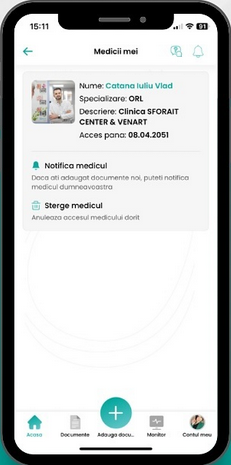
\includegraphics[width=0.45\textwidth]{Medvalet_1.png}} \quad
    \subfloat[Uploaded documents screen]{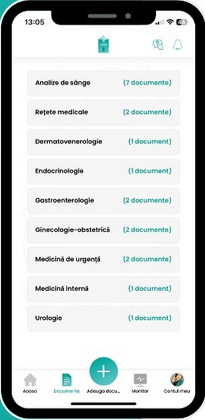
\includegraphics[width=0.45\textwidth]{Medvalet_2.png}}
    \caption{Medvalet screenshots}
    \label{fig:medvalet}
\end{figure}

\newpage

\subsubsection{Andaman7}

A mobile app developed by a Belgian-American eHealth company with the goal to improve doctor-patient communication, compliant with GDPR and HIPAA \parencite{andaman}.

\begin{table}[htbp]
\centering
    \begin{tabular}{|p{0.45\textwidth}|p{0.45\textwidth}|}
    \hline
    \textbf{Key Features/Benefits} & \textbf{Limitations/Drawbacks} \\ \hline
    \begin{itemize}
        \item Offers sections for personal information, medical history, allergies, vaccinations, medications, etc.
        \item Automatically collects health data from over 300 hospitals and clinics in the US and Europe.
        \item Supports input from diverse sources like hospitals, labs, smart devices or even manual input.
        \item Stores data locally on patients’ devices, ensuring privacy.
        \item Data sharing with QR codes and revokable access.
        \item AI tools for summarization, translation, and simplifying medical jargon.
    \end{itemize} &
    \begin{itemize}
        \item Requires patients and doctors to both create accounts.
        \item Does not extract data or values from uploaded documents like lab results.
        \item Limited to mobile platforms, which may limit usability for desktop-only users.
    \end{itemize} \\ \hline
    \end{tabular}
\caption{Andaman7 Features and Limitations}
\label{tab:andaman7}
\end{table}

\begin{figure}[ht]
    \centering
    \subfloat[PHR Sections screen]{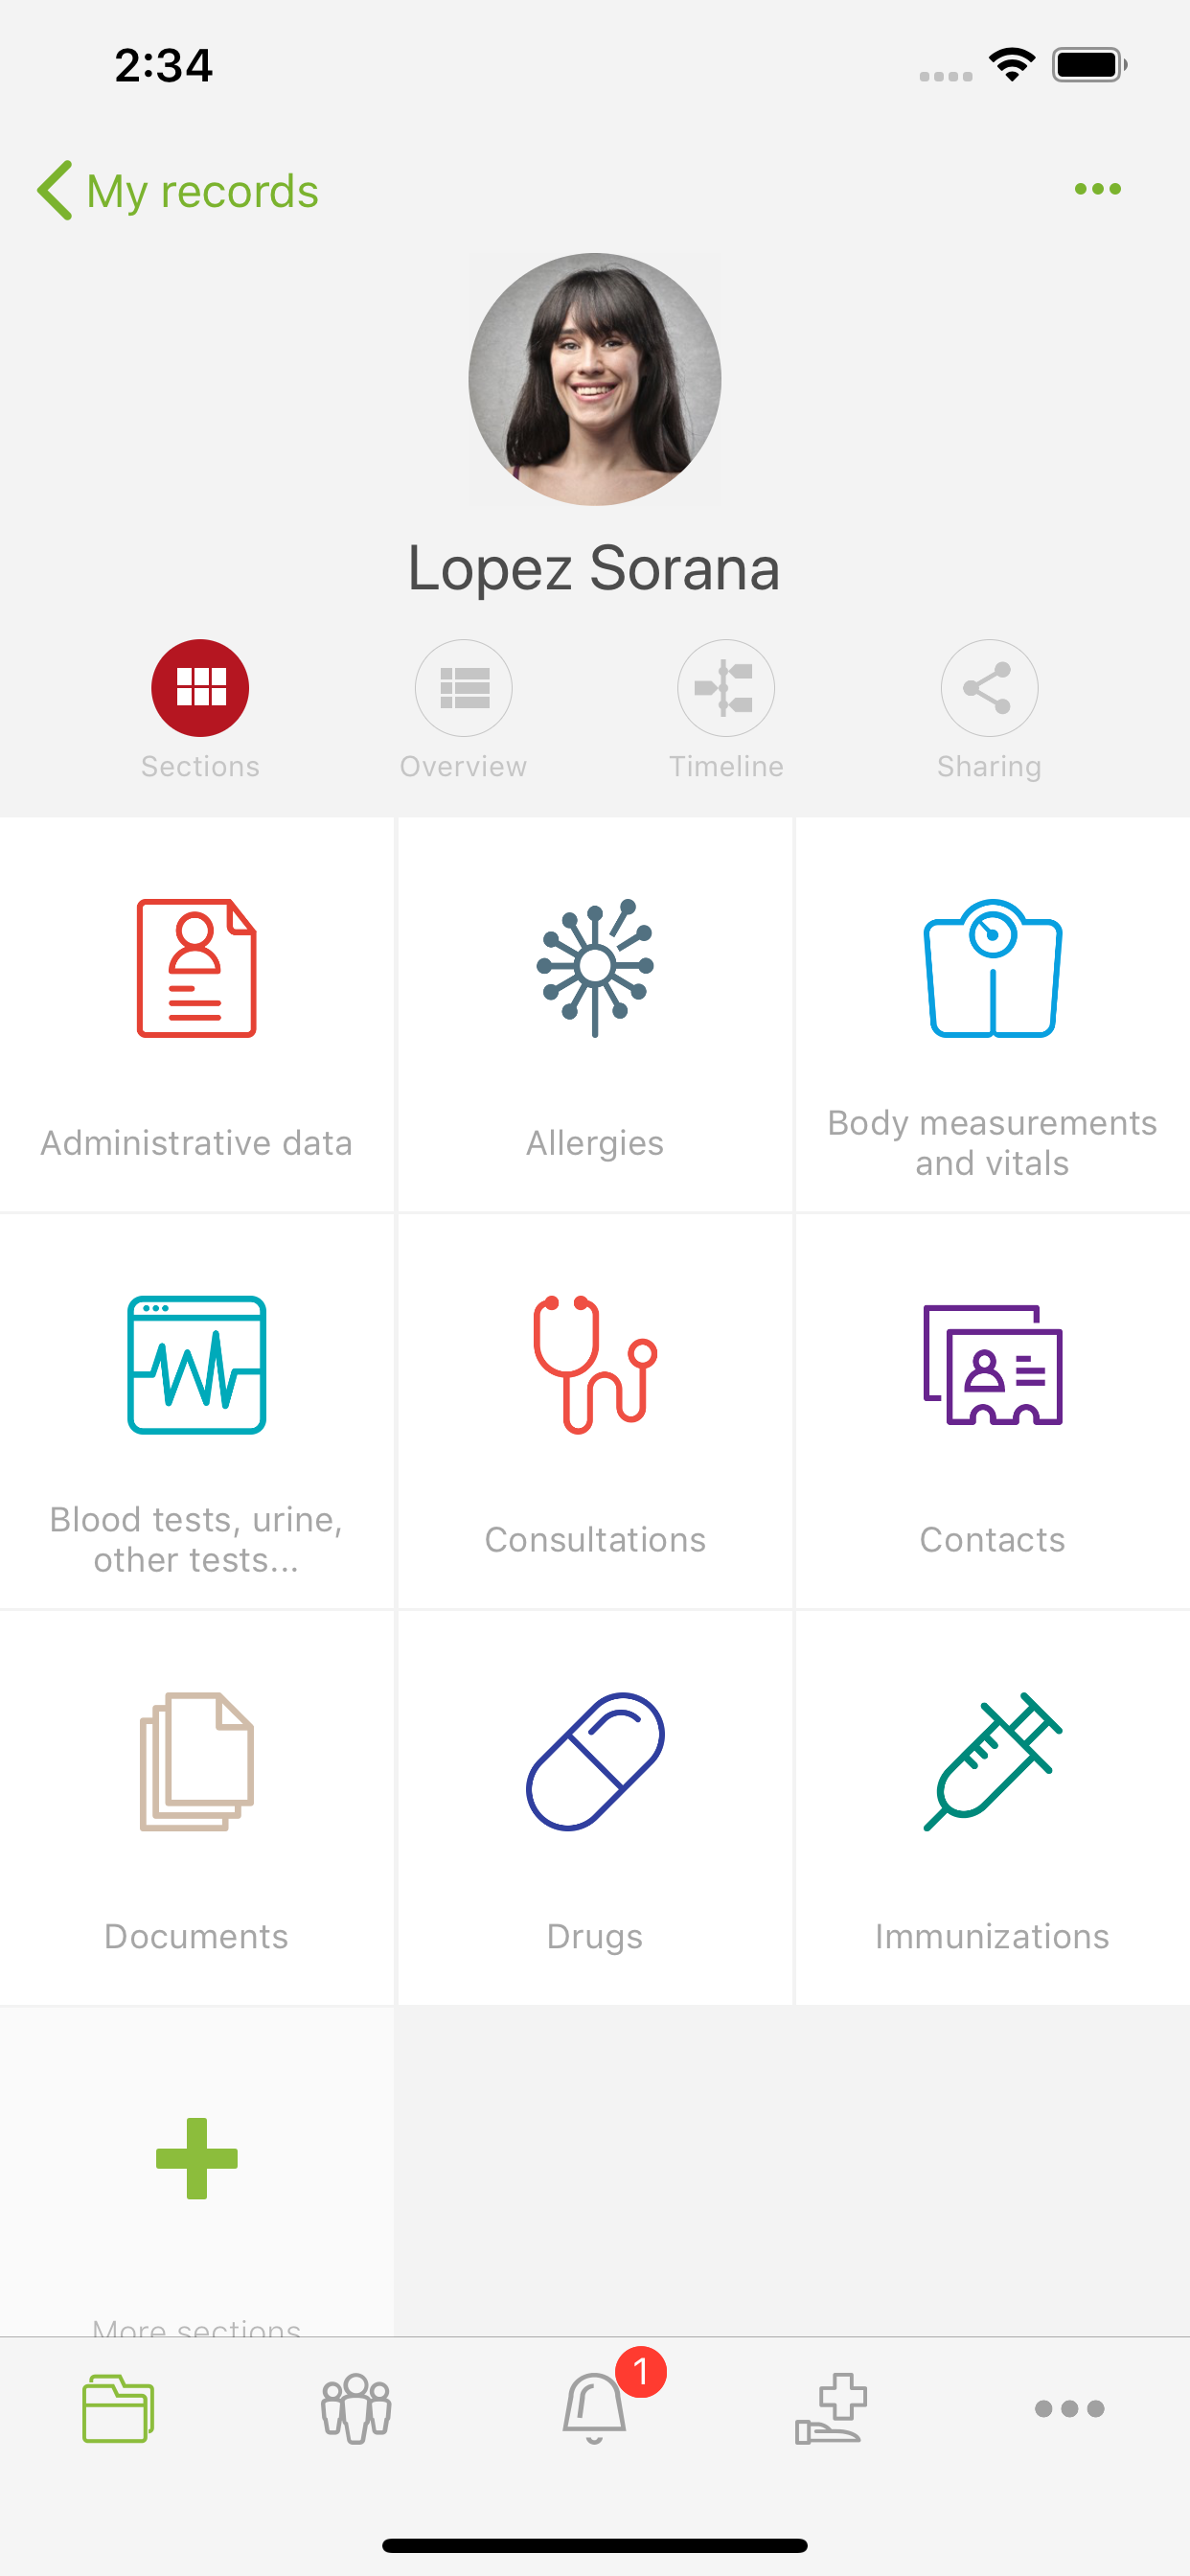
\includegraphics[width=0.45\textwidth]{Andaman_1.png}} \quad
    \subfloat[Documents section screen]{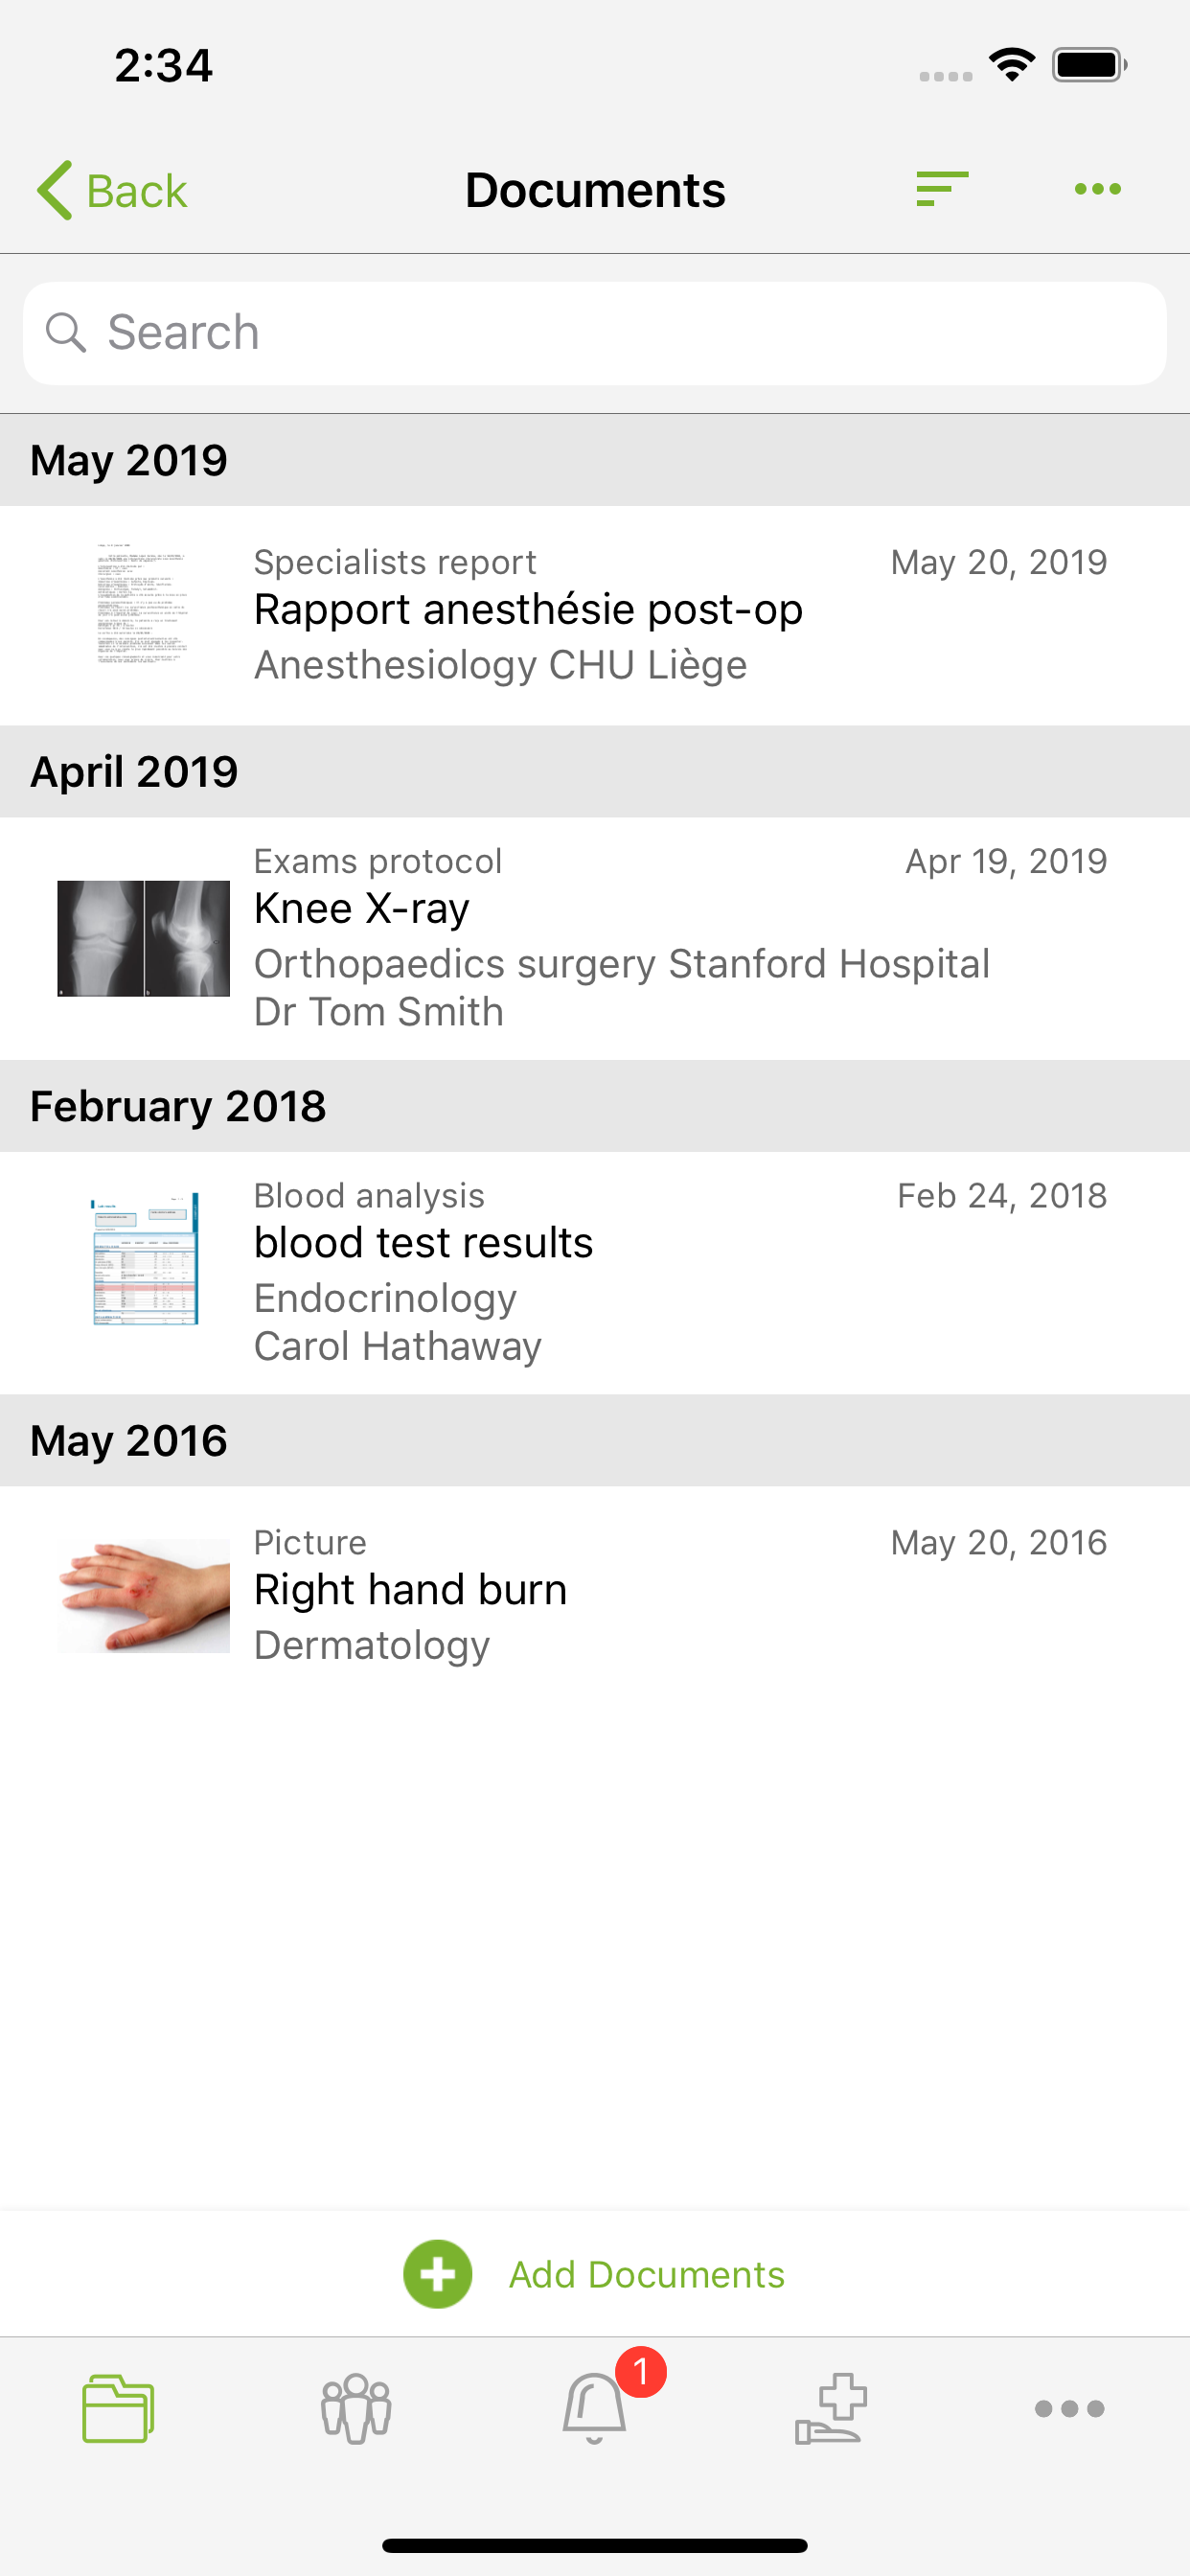
\includegraphics[width=0.45\textwidth]{Andaman_2.png}}
    \caption{Andaman7 screenshots}
    \label{fig:andaman7}
\end{figure}

\FloatBarrier

\subsubsection{Fasten Health}

An open-source, self-hosted electronic medical record aggregator with optional paid desktop versions for Windows and Mac \parencite{fasten}.

\begin{table}[h!]
\centering
    \begin{tabular}{|p{0.45\textwidth}|p{0.45\textwidth}|}
    \hline
    \textbf{Key Features/Benefits} & \textbf{Limitations/Drawbacks} \\ \hline
    \begin{itemize}
        \item Automatically aggregates records from multiple providers, like hospitals and labs.
        \item Supports self-hosting for complete control over data, stored locally.
        \item Compatible with protocols such as DICOM, FHIR, and OAuth2.
        \item Allows manual entry for allergies, vaccinations, and medications.
        \item Offers multiple dashboards with graphs to visualize health data.
        \item Supports multi-user functionality for families.
    \end{itemize} &
    \begin{itemize}
        \item Paid desktop versions may deter users.
        \item Manual data entry limited to new or existing encounters, complicating usage.
        \item Does not support OCR or automatic data extraction from documents.
        \item Lacks data-sharing capabilities with doctors.
        \item Requires technical expertise for self-hosting.
        \item Restricted to healthcare providers in the United States.
    \end{itemize} \\ \hline
    \end{tabular}
\caption{Fasten Health Features and Limitations}
\label{tab:fasten_health}
\end{table}

\begin{figure}[ht]
    \centering
    \subfloat[Fasten Health dashboard]{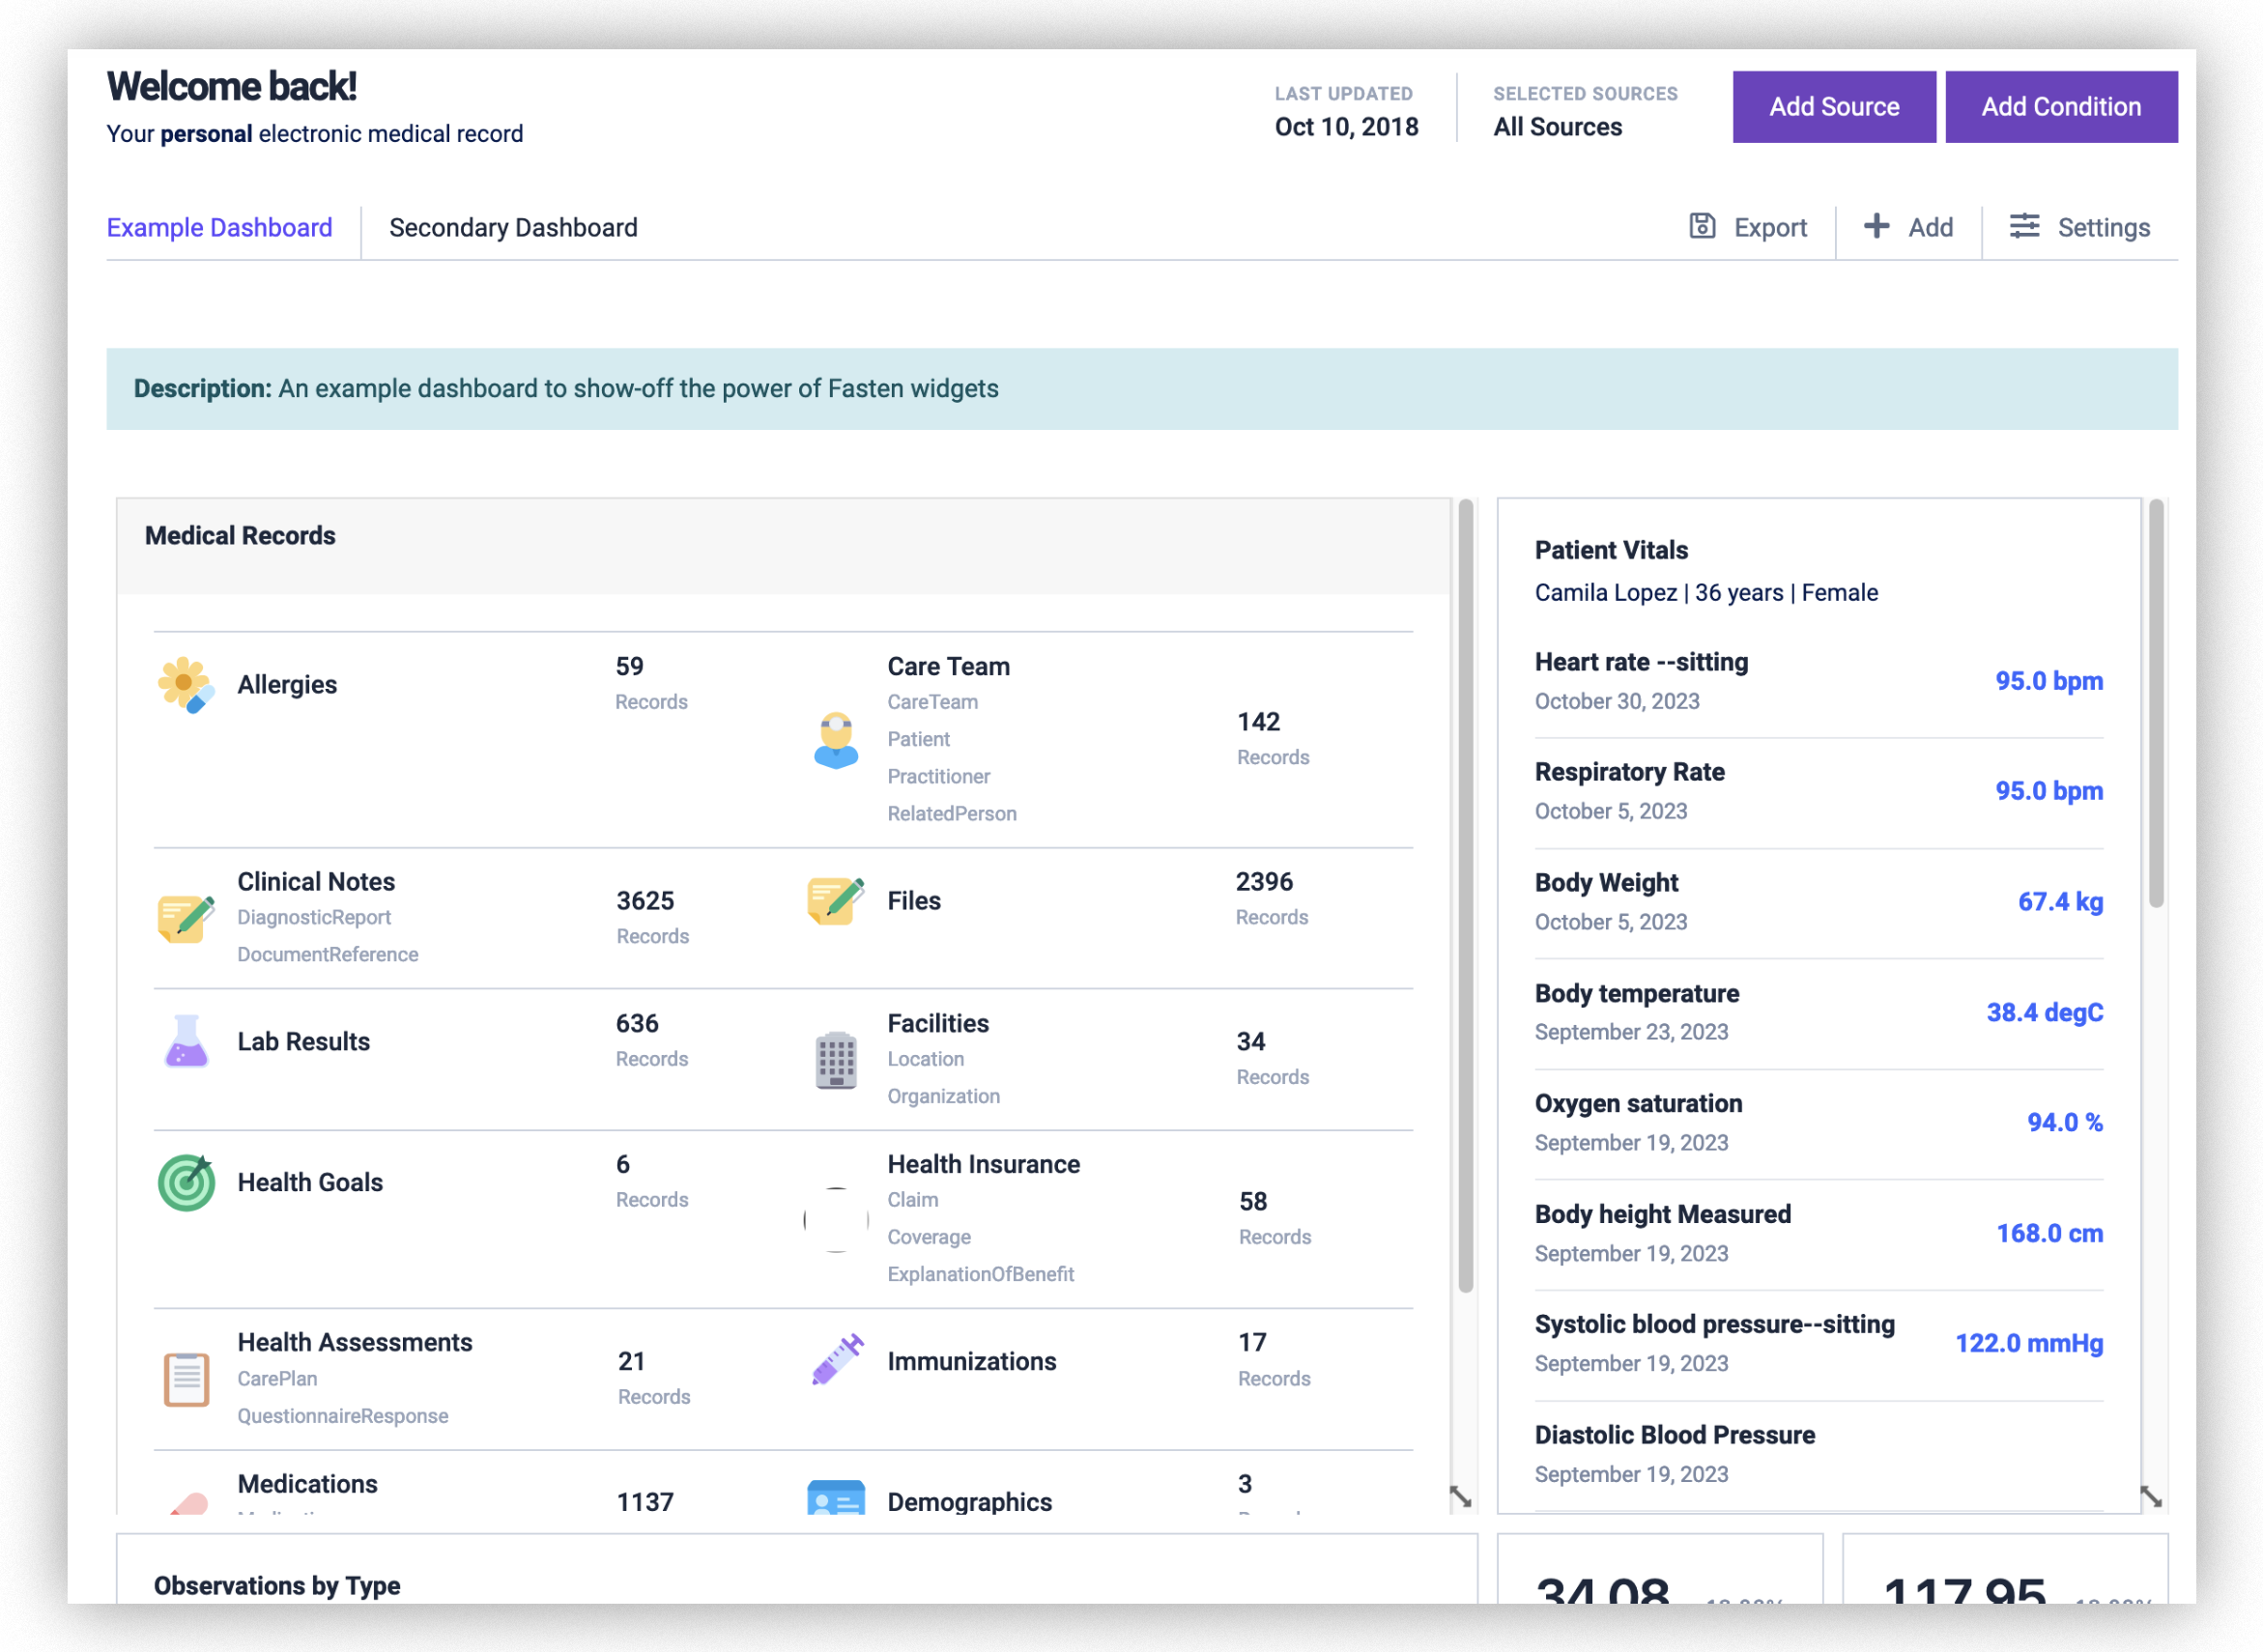
\includegraphics[width=0.75\textwidth]{fasten_1.png}\label{fig:fasten1}} 
    \hspace{0.05\textwidth} 
    \subfloat[Visit history screen]{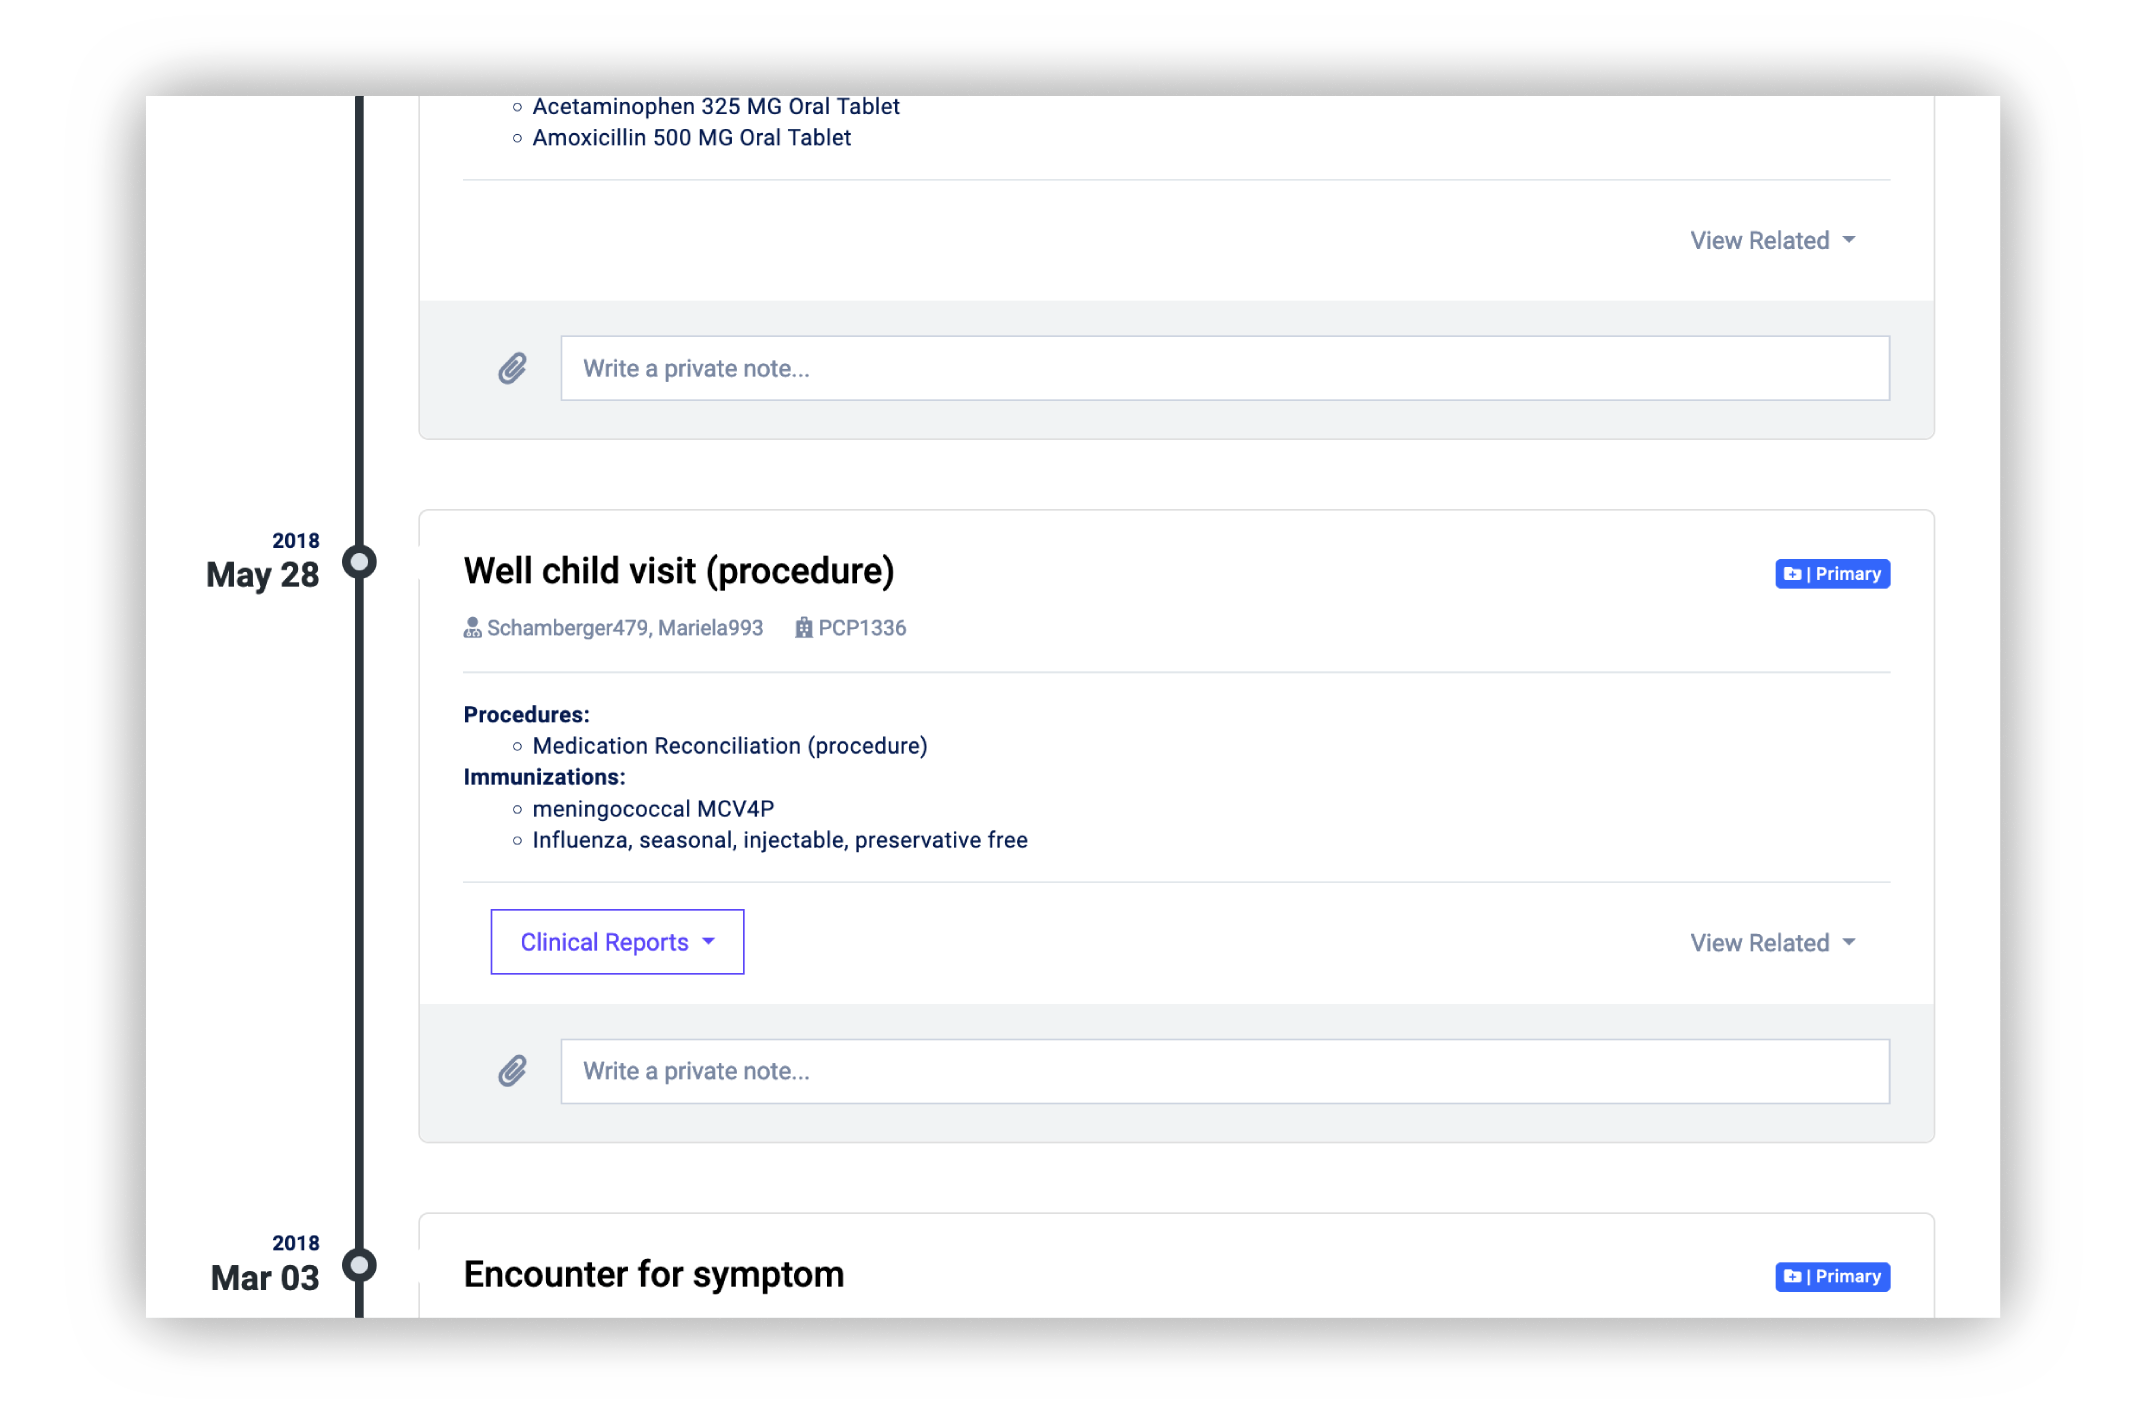
\includegraphics[scale=0.3]{fasten_2.png}\label{fig:fasten2}} 
    \caption{Overview of Fasten Health app features}
    \label{fig:fasten}
\end{figure}

